\documentclass[12pt]{labreport}
\usepackage[utf8]{inputenc}
%TC:macro \ref [option:inline,inline] [0]
%TC:macro \cite [option:text,text] [0]
%TC:macro \citep [option:text,text] [0]
%TC:group table 0 1 [0]
%TC:group tabularx 1 1 [0]

\title{Lab Report Template}
\subtitle{Subtitle}
\author{Dylan Chua}
\department{Mechanical Engineering}
\organisation{Imperial College London}
\date{November 2022}

\begin{document}
%TC:ignore
\frontmatter
\titlepage

\begin{abstract}
    Insert abstract text here. Lorem ipsum dolor sit amet, consectetur adipiscing elit, sed do eiusmod tempor incididunt ut labore et dolore magna aliqua. Lorem ipsum dolor sit amet, consectetur adipiscing elit, sed do eiusmod tempor incididunt ut labore et dolore magna aliqua. Lorem ipsum dolor sit amet, consectetur adipiscing elit, sed do eiusmod tempor incididunt ut labore et dolore magna aliqua.
\end{abstract}
\newpage

\tableofcontents
\newpage

\begin{nomen}
    \nomenclature[a]{\(E\)}{Young's modulus}
    \nomenclature[a]{\(F\)}{Force}
    \nomenclature[a]{\(L_0\)}{Initial gauge length}
    
    \nomenclature[ge]{$\varepsilon$}{Strain}

    \nomenclature[m]{BV}{Bridge Voltage}

    \nomenclature[z]{max}{Maximum}
\end{nomen}
%TC:endignore

\newpage
\mainmatter
\section{Introduction}
Something \cite{Bayer_etal_2013} in Table \ref{tab:gauge_pos}.

\section{Materials and methods}
\begin{table}[h]
    \centering
    \caption{Positions of strain gauges}
    \begin{tabularx}{\textwidth}{|>{\hsize=.20\hsize}X|>{\hsize=.80\hsize}X|} \hline
        Gauge & Position \\ \hline
        1, 2 & Edge of the hole, measure maximum strain \\ \hline
        3, 4, 5 & Same horizontal as 1 and 2, measure strain at varying distances \\ \hline
        6, 7, 8, 9 & Far from hole, measure remote strain \\ \hline
    \end{tabularx}
    \label{tab:gauge_pos}
\end{table}

\section{Results}

\begin{figure}[h]
    \centering
    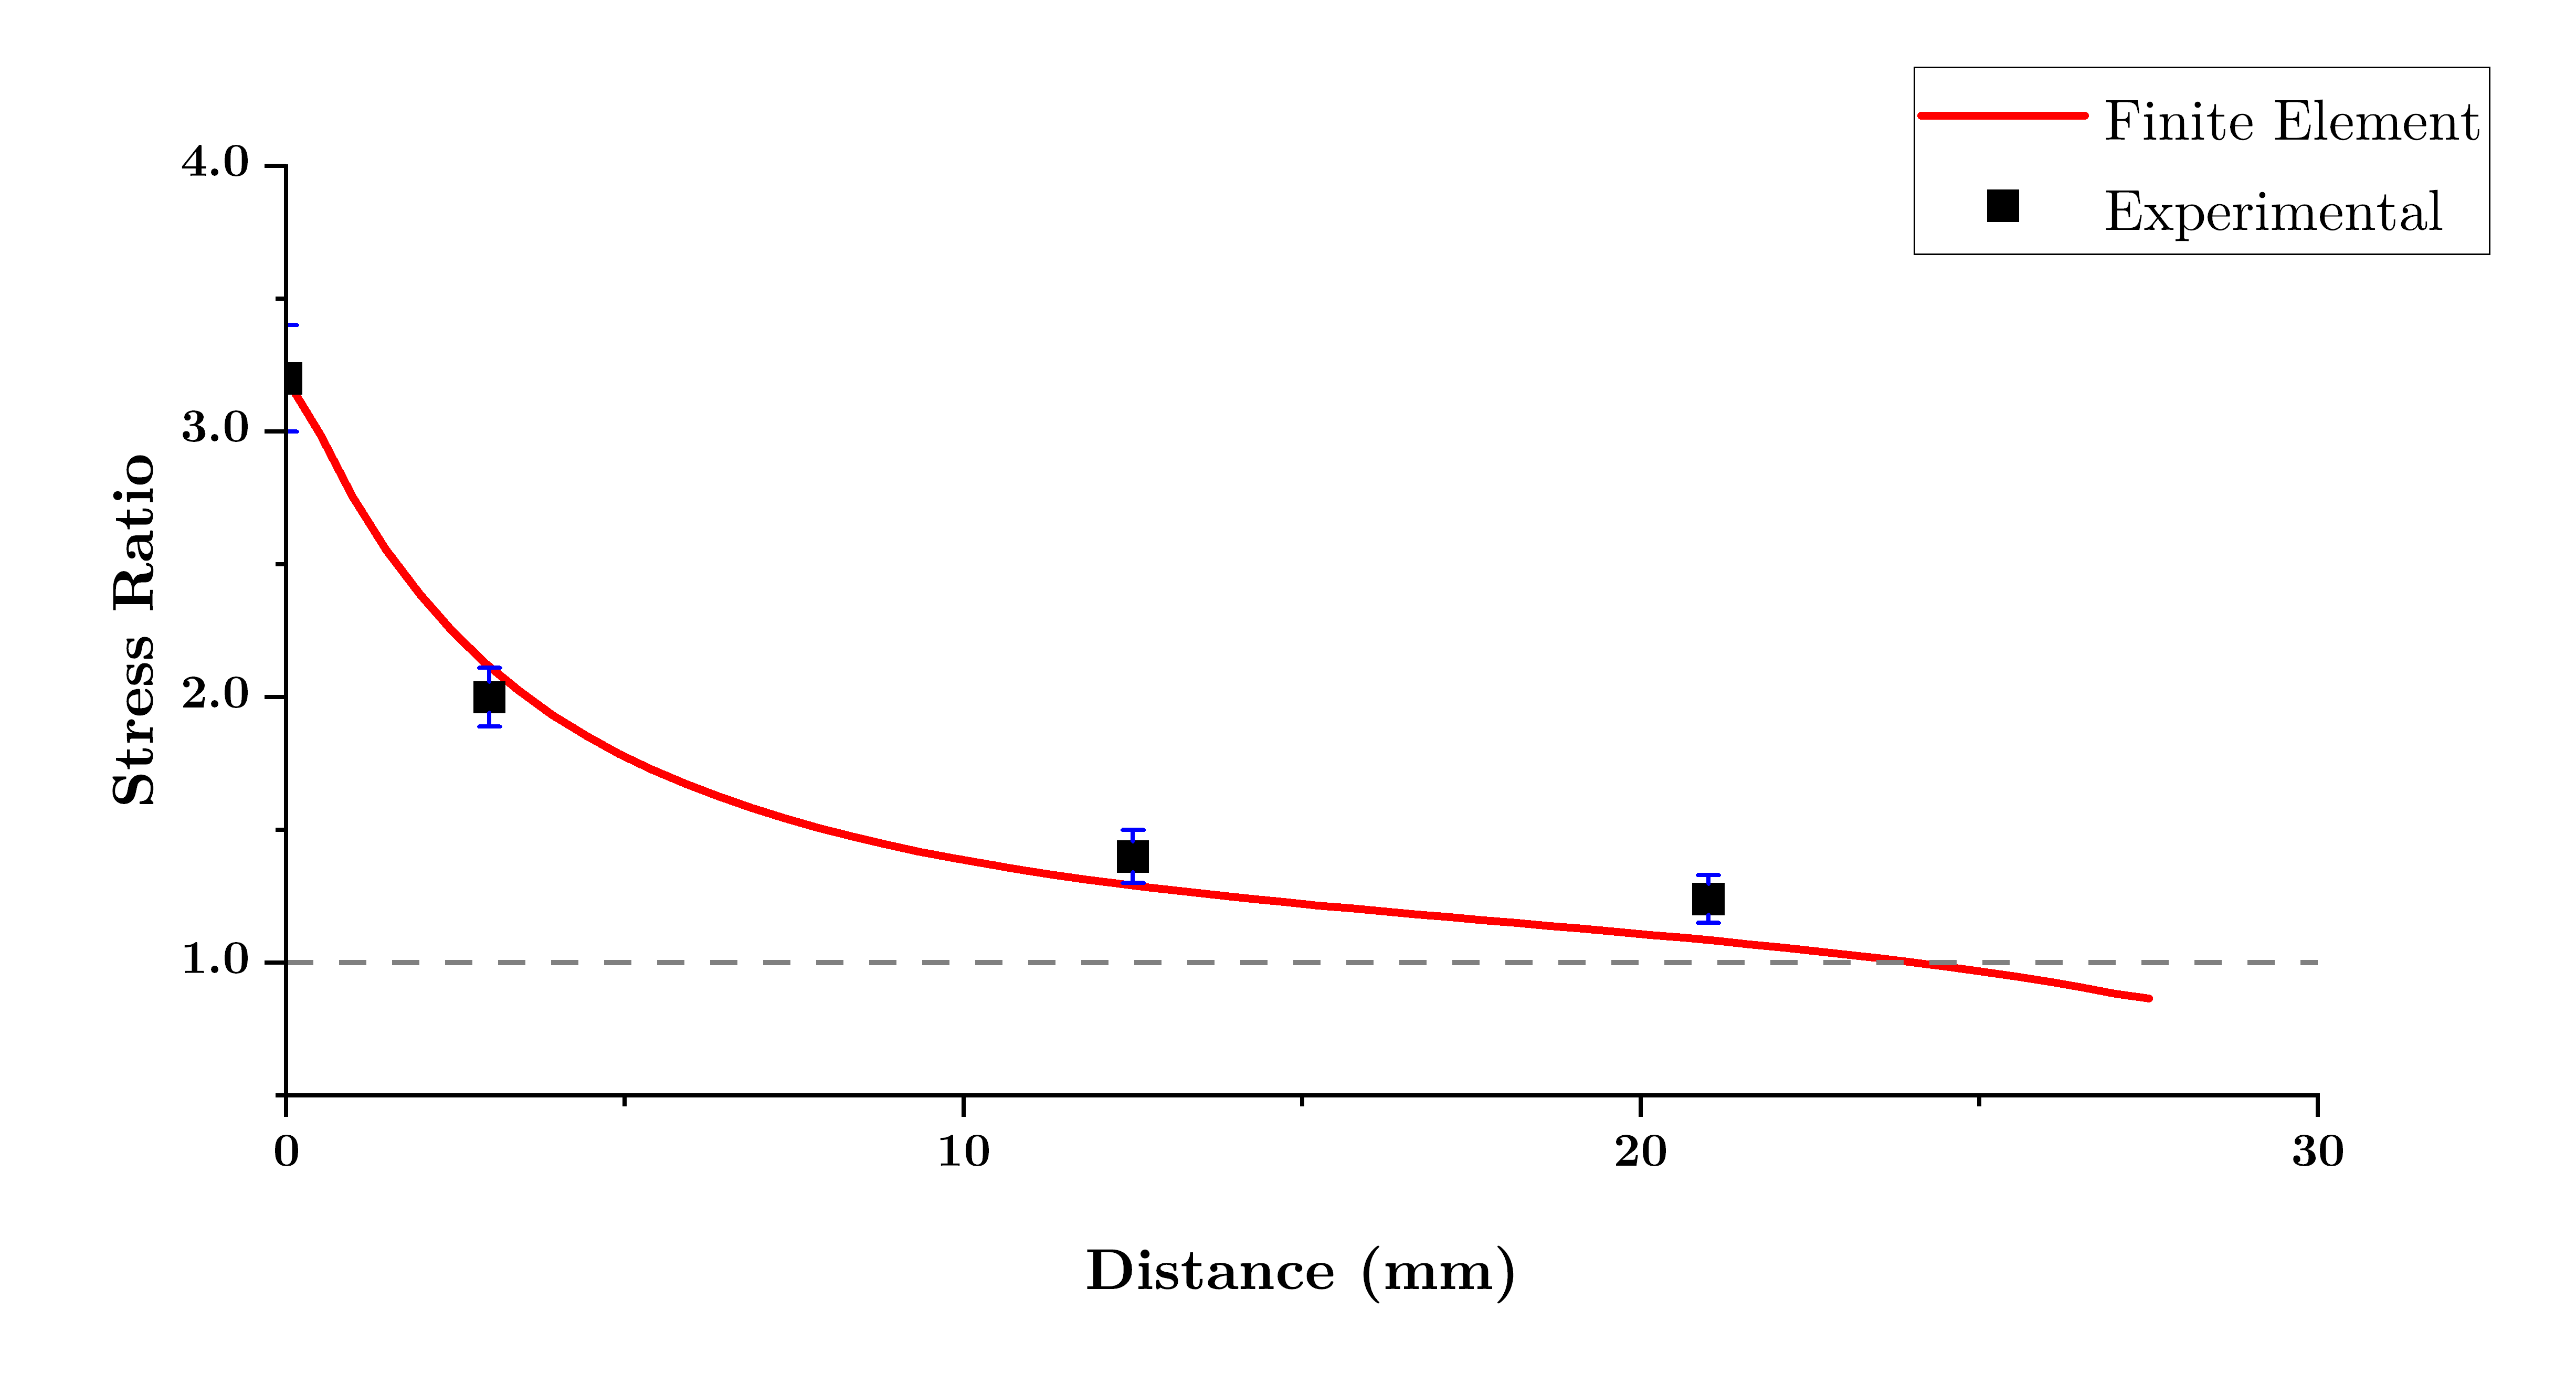
\includegraphics[width=\textwidth]{finite_element}
    \caption{Experimental values with FE data}
    \label{fig:finite_element}
\end{figure}

\section{Discussion}
\begin{equation}
\begin{split}
    \sigma_{nom} & = \frac{500\cdot5\cdot(30\cdot\frac{2\pi}{60})^2}{80\cdot10} \\
                 & = 30.84 \text{ MPa}
\end{split}
\end{equation}

\section{Conclusions}

%TC:ignore
\section{Acknowledgements}

\bibliography{cite}

\backmatter
\begin{appendices}
\appendix
\addtocontents{toc}{\protect\setcounter{tocdepth}{1}}
\section{first appendix}

    
\end{appendices}

\end{document}
